\documentclass[11pt,a4paper]{article}

% ============================================================
% Packages
% ============================================================
\usepackage[utf8]{inputenc}
\usepackage[T1]{fontenc}
\usepackage[portuguese]{babel}
\usepackage{helvet}
\renewcommand{\familydefault}{\sfdefault}
\usepackage[margin=2.5cm]{geometry}
\usepackage{setspace}
\onehalfspacing
\usepackage{graphicx}
\usepackage{float}
\usepackage{booktabs}
\usepackage{tabularx}
\usepackage{hyperref}
\usepackage{xcolor}
\usepackage{enumitem}
\usepackage{listings}
\usepackage{fancyhdr}

% ============================================================
% Header/Footer
% ============================================================
\pagestyle{fancy}
\fancyhf{}
\fancyhead[L]{\footnotesize\textit{Data Science and Analytics -- 2026}}
\fancyfoot[R]{\footnotesize\thepage}
\renewcommand{\headrulewidth}{0.4pt}

% ============================================================
% JSON listing
% ============================================================
\lstdefinestyle{json}{
  basicstyle=\footnotesize\ttfamily,
  breaklines=true,
  frame=single,
  backgroundcolor=\color{gray!5},
}

% ============================================================
\begin{document}

% ============================================================
% Folha de rosto
% ============================================================
\begin{titlepage}
\centering
\vspace*{3cm}
{\LARGE\bfseries Constru\c{c}\~{a}o de corpus multi-camada de coment\'{a}rios b\'{i}blicos patr\'{i}sticos}
\vspace{1.5cm}

{\large Iury Anderson Fernandes Coelho\textsuperscript{1}}
\vspace{0.3cm}

{\small\textsuperscript{1}MBA Data Science and Analytics -- USP/ESALQ}
\vspace{2cm}

{\large Orientador: [Nome do Orientador]}
\vfill
{\small 2026}
\end{titlepage}

% ============================================================
% Resumo
% ============================================================
\section*{Resumo}
\begin{singlespace}
Este trabalho descreve a constru\c{c}\~{a}o de um corpus estruturado de coment\'{a}rios b\'{i}blicos patr\'{i}sticos contendo 31.218 arquivos de vers\'{i}culos e 55.925 coment\'{a}rios individuais, cobrindo 66 livros b\'{i}blicos e mais de 100 autores do per\'{i}odo AD~100--1700. O corpus foi constru\'{i}do atrav\'{e}s de um pipeline de quatro etapas: extra\c{c}\~{a}o h\'{i}brida via \textit{web scraping} (Firecrawl + BeautifulSoup), limpeza autom\'{a}tica de codifica\c{c}\~{a}o utilizando a biblioteca \texttt{ftfy}, tradu\c{c}\~{a}o autom\'{a}tica para portugu\^{e}s brasileiro via GPT-4o-mini e enriquecimento estruturado por intelig\^{e}ncia artificial. A etapa de limpeza corrigiu 14.906 problemas de codifica\c{c}\~{a}o e reduziu o tamanho do corpus em 33\%, de 195~MB para 131~MB, sem perda de conte\'{u}do. O dataset est\'{a} dispon\'{i}vel publicamente sob licen\c{c}a CC~BY~4.0.
\end{singlespace}

\vspace{0.3cm}
\noindent\textbf{Palavras-chave:} corpus patr\'{i}stico, pipeline de dados, limpeza de texto, processamento de linguagem natural, \textit{web scraping}

% ============================================================
% 1. Consideracoes Iniciais
% ============================================================
\section{Considera\c{c}\~{o}es iniciais}

Coment\'{a}rios b\'{i}blicos patr\'{i}sticos s\~{a}o textos exeg\'{e}ticos produzidos pelos Pais da Igreja entre os s\'{e}culos II e XVIII. Esses textos representam mais de 1.600 anos de tradi\c{c}\~{a}o interpretativa e constituem uma fonte hist\'{o}rica de valor significativo para estudos teol\'{o}gicos, lingu\'{i}sticos e computacionais. Autores como Agostinho de Hipona (AD~430), Jo\~{a}o Cris\'{o}stomo (AD~407), Beda (AD~735) e Jer\^{o}nimo (AD~420) produziram coment\'{a}rios vers\'{i}culo a vers\'{i}culo que permanecem referência na tradi\c{c}\~{a}o crist\~{a}.

Apesar da import\^{a}ncia desses textos, sua disponibilidade em formato estruturado para processamento computacional \'{e} limitada. Plataformas como o CatenaBible.com disponibilizam coment\'{a}rios em formato web, por\'{e}m sem estrutura\c{c}\~{a}o adequada para an\'{a}lises de processamento de linguagem natural [NLP] ou recupera\c{c}\~{a}o de informa\c{c}\~{a}o [IR].

O objetivo deste trabalho \'{e} apresentar a constru\c{c}\~{a}o de um corpus multi-camada de coment\'{a}rios patr\'{i}sticos, desde a extra\c{c}\~{a}o autom\'{a}tica at\'{e} o enriquecimento por intelig\^{e}ncia artificial, com \^{e}nfase na rastreabilidade, reprodutibilidade e qualidade dos dados.

% ============================================================
% 2. Material e Metodos
% ============================================================
\section{Material e m\'{e}todos}

\subsection{Fonte de dados}

Os coment\'{a}rios foram extra\'{i}dos do CatenaBible.com, uma plataforma que disponibiliza textos patr\'{i}sticos organizados vers\'{i}culo a vers\'{i}culo. Os textos originais s\~{a}o de dom\'{i}nio p\'{u}blico, produzidos entre AD~100 e AD~1700. A fonte cobre o c\^{a}non completo (66 livros), incluindo livros deuterocan\^{o}nicos.

\subsection{Arquitetura do pipeline}

O pipeline \'{e} composto por quatro camadas numeradas sequencialmente. Cada camada \'{e} produzida por um \'{u}nico script, e cada script mapeia exatamente uma transi\c{c}\~{a}o entre camadas (Figura~\ref{fig:pipeline}).

\begin{figure}[H]
\centering
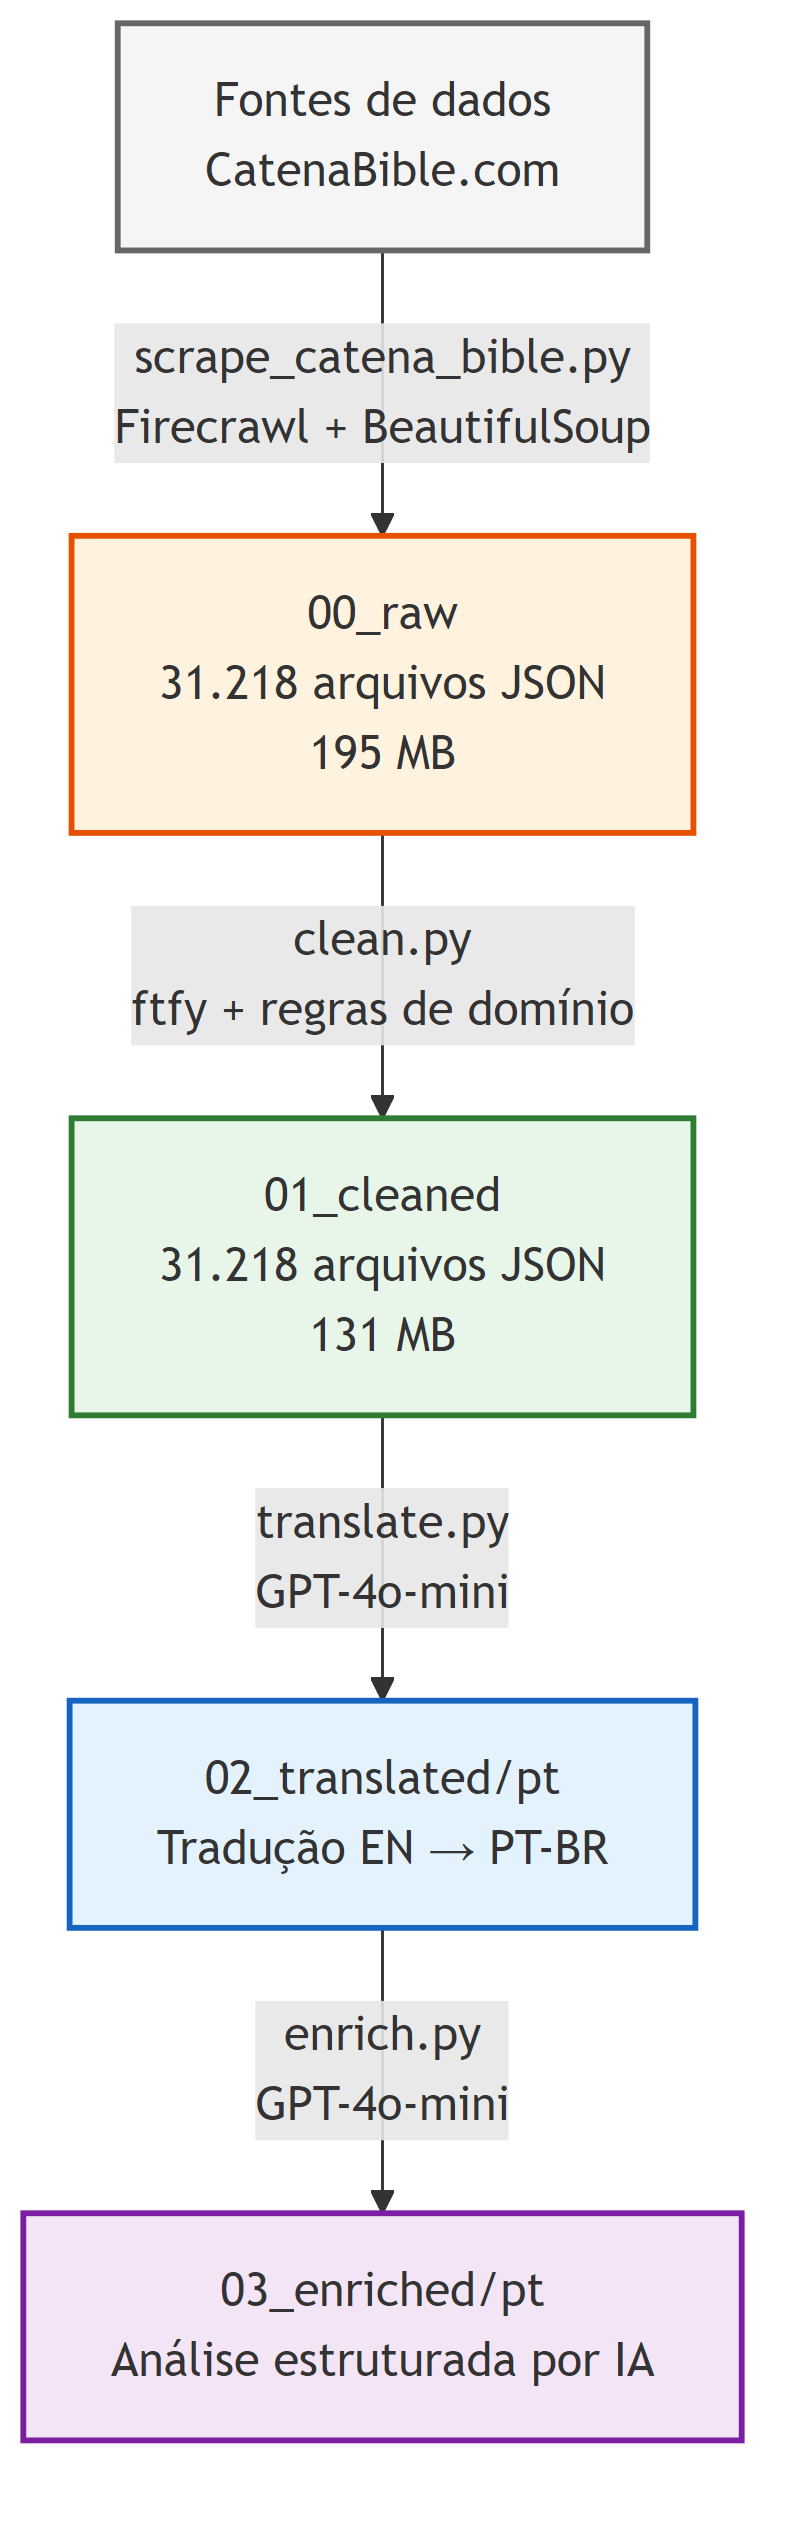
\includegraphics[width=0.75\textwidth]{figures/pipeline.png}
\caption{Arquitetura do pipeline de processamento em quatro camadas}
\label{fig:pipeline}

Fonte: Resultados originais da pesquisa
\end{figure}

\subsection{Etapa 0: extra\c{c}\~{a}o (\textit{web scraping})}

A extra\c{c}\~{a}o utiliza uma abordagem h\'{i}brida combinando dois motores (Figura~\ref{fig:scraping}):

\begin{itemize}[leftmargin=1.25cm]
\item \textbf{Firecrawl}: navega\c{c}\~{a}o e extra\c{c}\~{a}o de conte\'{u}do completo, incluindo conte\'{u}do de links secund\'{a}rios (``Go to Commentary'')
\item \textbf{BeautifulSoup}: \textit{parsing} estruturado do HTML para identificar autor, per\'{i}odo e conte\'{u}do de cada coment\'{a}rio
\end{itemize}

O script implementa deduplicação por hash (primeiros 500 caracteres + URL) para evitar duplicatas entre os dois motores, e \textit{checkpointing} por cap\'{i}tulo para permitir retomada em caso de interrup\c{c}\~{a}o. O resultado \'{e} um arquivo JSON por vers\'{i}culo contendo todos os coment\'{a}rios dispon\'{i}veis.

\begin{figure}[H]
\centering
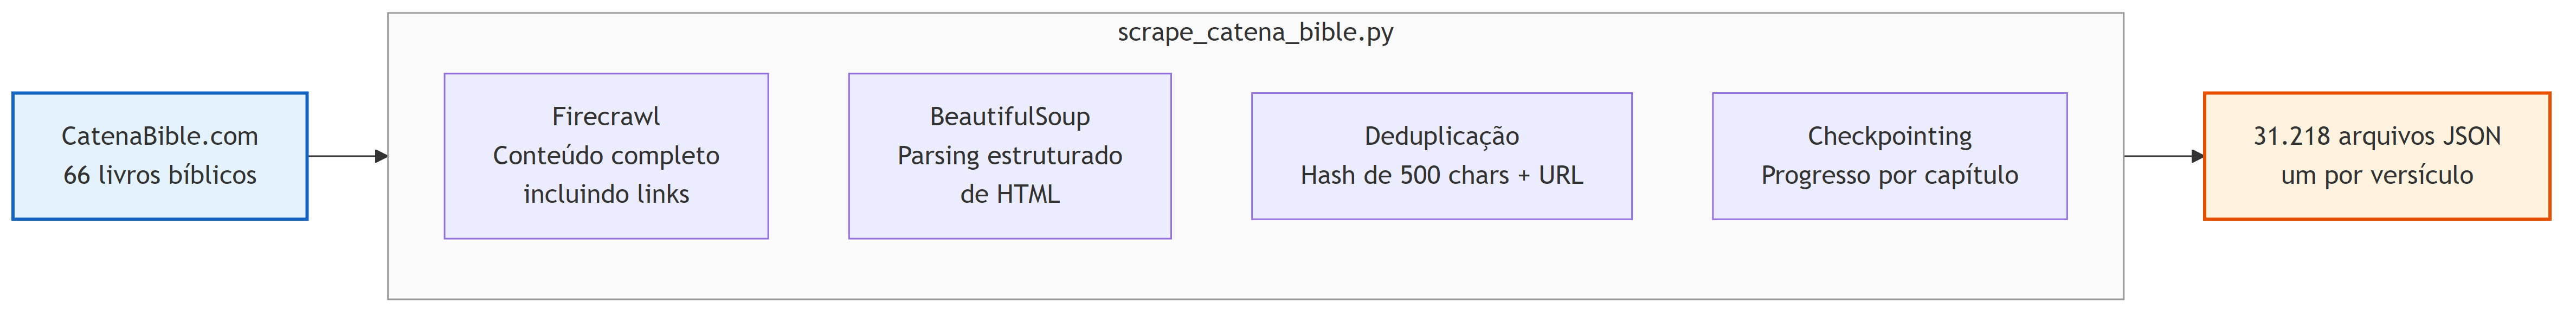
\includegraphics[width=0.75\textwidth]{figures/scraping-architecture.png}
\caption{Arquitetura do \textit{web scraping} h\'{i}brido}
\label{fig:scraping}

Fonte: Resultados originais da pesquisa
\end{figure}

\subsection{Etapa 1: limpeza de dados}

A limpeza \'{e} a etapa mais cr\'{i}tica do pipeline. Utiliza a biblioteca \texttt{ftfy} (Speer, 2019) como motor principal para corre\c{c}\~{a}o de problemas de codifica\c{c}\~{a}o, combinada com regras de dom\'{i}nio espec\'{i}ficas (Figura~\ref{fig:cleaning}).

\begin{figure}[H]
\centering
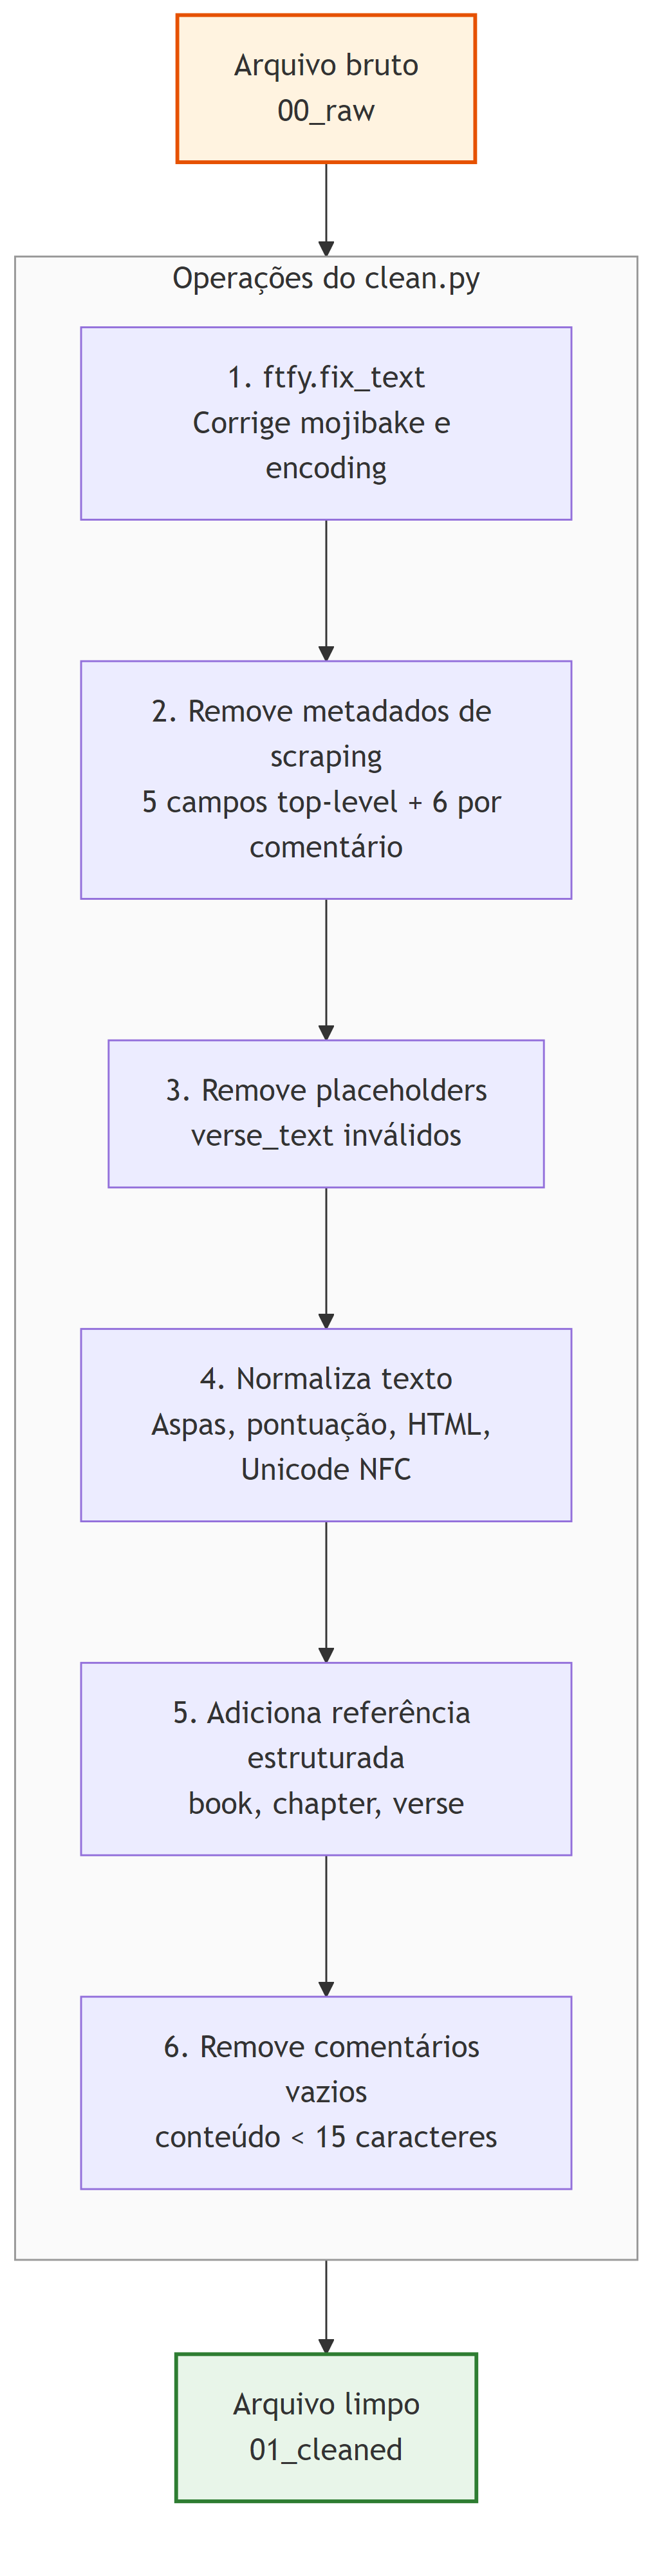
\includegraphics[width=0.65\textwidth]{figures/cleaning-process.png}
\caption{Opera\c{c}\~{o}es realizadas na etapa de limpeza}
\label{fig:cleaning}

Fonte: Resultados originais da pesquisa
\end{figure}

A biblioteca \texttt{ftfy} detecta e corrige automaticamente \textit{mojibake} --- texto que foi codificado em UTF-8 mas decodificado incorretamente como Latin-1 ou CP-1252. Al\'{e}m disso, normaliza entidades HTML residuais, liga\c{c}\~{o}es tipogr\'{a}ficas e caracteres de largura total.

As regras de dom\'{i}nio adicionais incluem:

\begin{enumerate}[leftmargin=1.25cm]
\item Remo\c{c}\~{a}o de 5 campos de metadados de \textit{scraping} do n\'{i}vel superior (\texttt{scraped\_with}, \texttt{extraction\_date}, \texttt{source\_url}, \texttt{full\_content\_fetched}, \texttt{methodology})
\item Remo\c{c}\~{a}o de 6 campos por coment\'{a}rio (\texttt{commentary\_number}, \texttt{reading\_time}, \texttt{source\_url}, \texttt{full\_content\_url}, \texttt{content\_type}, \texttt{extraction\_method})
\item Remo\c{c}\~{a}o de \textit{placeholders} no campo \texttt{verse\_text} (padr\~{a}o ``Verse text for \{REF\}'')
\item Corre\c{c}\~{a}o de aspas duplicadas, pontua\c{c}\~{a}o inicial \'{o}rf\~{a} e \textit{backslashes} residuais
\item Remo\c{c}\~{a}o de tags HTML remanescentes
\item Adi\c{c}\~{a}o de campos de refer\^{e}ncia normalizados (\texttt{book}, \texttt{chapter}, \texttt{verse}), parseados do nome do arquivo
\item Normaliza\c{c}\~{a}o Unicode para forma NFC
\end{enumerate}

O resultado \'{e} um JSON enxuto contendo apenas os campos relevantes para pesquisa: refer\^{e}ncia b\'{i}blica, status, contagem e lista de coment\'{a}rios (autor, per\'{i}odo, conte\'{u}do).

\subsection{Etapa 2: tradu\c{c}\~{a}o autom\'{a}tica}

A tradu\c{c}\~{a}o do ingl\^{e}s para o portugu\^{e}s brasileiro utiliza o modelo GPT-4o-mini da OpenAI, com um gloss\'{a}rio teol\'{o}gico de 14 termos embutido no \textit{prompt} para garantir consist\^{e}ncia terminol\'{o}gica (por exemplo, \textit{Trinity} $\rightarrow$ Trindade, \textit{grace} $\rightarrow$ gra\c{c}a, \textit{incarnation} $\rightarrow$ encarna\c{c}\~{a}o).

O script suporta m\'{u}ltiplos idiomas por \textit{design}: o par\^{a}metro \texttt{--lang} define o idioma alvo, permitindo que o pipeline seja reutilizado para espanhol, franc\^{e}s ou outros idiomas sem modifica\c{c}\~{a}o.

Os arquivos traduzidos cont\^{e}m apenas os campos essenciais: \texttt{verse\_reference} e uma lista de coment\'{a}rios com \texttt{author}, \texttt{period} e \texttt{content\_pt}. Metadados de tradu\c{c}\~{a}o (modelo, data) s\~{a}o armazenados em um arquivo separado (\texttt{translation\_metadata.json}).

\subsection{Etapa 3: enriquecimento por IA}

O enriquecimento adiciona an\'{a}lise estruturada a cada coment\'{a}rio traduzido, utilizando GPT-4o-mini com um \textit{system prompt} especializado em teologia patr\'{i}stica. Para cada coment\'{a}rio, quatro campos s\~{a}o gerados:

\begin{itemize}[leftmargin=1.25cm]
\item \texttt{ai\_summary}: resumo em uma frase, resumo expandido e pontos-chave
\item \texttt{argumentative\_structure}: tese, argumentos, obje\c{c}\~{o}es e conclus\~{a}o
\item \texttt{theological\_analysis}: doutrinas, tradi\c{c}\~{o}es (Alexandrina, Antioquena, Latina), m\'{e}todo teol\'{o}gico e controv\'{e}rsias
\item \texttt{spiritual\_insight}: tema central e reflex\~{a}o pr\'{a}tica
\end{itemize}

Esta etapa \'{e} executada seletivamente, dado o custo superior por arquivo (\$0,01 vs \$0,001 da tradu\c{c}\~{a}o).

\subsection{Valida\c{c}\~{a}o e ferramentas auxiliares}

O pipeline inclui tr\^{e}s scripts de valida\c{c}\~{a}o:

\begin{itemize}[leftmargin=1.25cm]
\item \texttt{validate\_schema.py}: valida cada arquivo contra o esquema esperado, identificando campos ausentes, conte\'{u}dos vazios e inconsist\^{e}ncias de contagem
\item \texttt{gap\_audit.py}: compara duas camadas para detectar arquivos ausentes
\item \texttt{generate\_manifest.py}: gera invent\'{a}rio completo com contagem por livro, n\'{u}mero de coment\'{a}rios e anomalias
\end{itemize}

% ============================================================
% 3. Resultados e Discussao
% ============================================================
\section{Resultados e discuss\~{a}o}

\subsection{Escala do corpus}

O corpus resultante cont\'{e}m 31.218 arquivos de vers\'{i}culos cobrindo os dois testamentos da B\'{i}blia e livros deuterocan\^{o}nicos (Tabela~\ref{tab:stats}).

\begin{table}[H]
\centering
\caption{Estat\'{i}sticas gerais do corpus}
\label{tab:stats}
\begin{tabularx}{0.75\textwidth}{Xr}
\toprule
M\'{e}trica & Valor \\
\midrule
Total de arquivos de vers\'{i}culo & 31.218 \\
Coment\'{a}rios individuais & 55.925 \\
Vers\'{i}culos com coment\'{a}rios & 22.537 \\
Vers\'{i}culos sem coment\'{a}rios & 8.681 \\
Livros b\'{i}blicos cobertos & 66 \\
Autores \'{u}nicos & 100+ \\
Per\'{i}odo temporal & AD 100 -- 1700 \\
\bottomrule
\end{tabularx}

Fonte: Resultados originais da pesquisa
\end{table}

A Tabela~\ref{tab:coverage} apresenta a distribui\c{c}\~{a}o dos arquivos por categoria b\'{i}blica. Os livros hist\'{o}ricos do Antigo Testamento representam a maior concentra\c{c}\~{a}o de coment\'{a}rios (6.851 arquivos), seguidos pelo Pentateuco (5.851) e pela literatura sapiencial (4.785).

\begin{table}[H]
\centering
\caption{Distribui\c{c}\~{a}o dos arquivos por categoria b\'{i}blica}
\label{tab:coverage}
\begin{tabularx}{0.75\textwidth}{Xlr}
\toprule
Categoria & Testamento & Arquivos \\
\midrule
Livros Hist\'{o}ricos & AT & 6.851 \\
Pentateuco & AT & 5.851 \\
Literatura Sapiencial & AT & 4.785 \\
Profetas Maiores & AT & 4.544 \\
Profetas Menores & AT & 1.122 \\
Deuterocan\^{o}nicos & AT & 167 \\
Evangelhos & NT & 3.779 \\
Ep\'{i}stolas Paulinas & NT & 2.110 \\
Atos dos Ap\'{o}stolos & NT & 1.007 \\
Ep\'{i}stolas Gerais & NT & 734 \\
Apocalipse & NT & 404 \\
\midrule
\textbf{Total} & & \textbf{31.354} \\
\bottomrule
\end{tabularx}

Fonte: Resultados originais da pesquisa
\end{table}

Os cinco autores mais frequentes no corpus s\~{a}o George Leo Haydock (AD~1849), Jo\~{a}o Cris\'{o}stomo (AD~407), Agostinho de Hipona (AD~430), Greg\'{o}rio Magno (AD~604) e Tertuliano de Cartago (AD~220), abrangendo tanto a tradi\c{c}\~{a}o oriental quanto a ocidental.

\subsection{Resultados da limpeza}

A execu\c{c}\~{a}o do script de limpeza sobre o corpus completo produziu os resultados apresentados na Tabela~\ref{tab:cleaning}.

\begin{table}[H]
\centering
\caption{Resultados da execu\c{c}\~{a}o do \texttt{clean.py} sobre o corpus completo}
\label{tab:cleaning}
\begin{tabularx}{0.75\textwidth}{Xr}
\toprule
M\'{e}trica & Valor \\
\midrule
Arquivos processados & 31.218 \\
Corre\c{c}\~{o}es de codifica\c{c}\~{a}o (ftfy) & 14.906 \\
Campos de metadados removidos & 156.090 \\
Coment\'{a}rios removidos (conte\'{u}do vazio) & 1 \\
Redu\c{c}\~{a}o de tamanho & 33\% (195 MB $\rightarrow$ 131 MB) \\
Erros de processamento & 0 \\
Tempo de execu\c{c}\~{a}o & 119 segundos \\
\bottomrule
\end{tabularx}

Fonte: Resultados originais da pesquisa
\end{table}

A biblioteca \texttt{ftfy} corrigiu 14.906 problemas de codifica\c{c}\~{a}o automaticamente, sem falsos positivos. A verifica\c{c}\~{a}o em uma amostra de 1.000 arquivos confirmou zero perda de conte\'{u}do: todos os 1.753 coment\'{a}rios da amostra foram preservados integralmente ap\'{o}s a limpeza, com 253 normaliza\c{c}\~{o}es de texto (corre\c{c}\~{o}es de codifica\c{c}\~{a}o) e nenhum caso de truncamento.

A remo\c{c}\~{a}o de 156.090 campos de metadados de \textit{scraping} resultou em uma redu\c{c}\~{a}o de 33\% no tamanho total do corpus, produzindo arquivos JSON enxutos contendo apenas os campos relevantes para pesquisa.

\subsection{Estrutura dos dados resultantes}

O formato final de cada arquivo na camada limpa (01\_cleaned) cont\'{e}m a seguinte estrutura:

\begin{lstlisting}[style=json]
{
  "verse_reference": "ACTS 1:1",
  "book": "acts",
  "chapter": 1,
  "verse": 1,
  "commentary_status": "available",
  "total_commentaries": 12,
  "commentaries": [
    {
      "author": "Bede",
      "period": "AD735",
      "content": "primeiro discurso: Ou seja, ..."
    }
  ]
}
\end{lstlisting}

\subsection{Garantias do pipeline}

O pipeline oferece tr\^{e}s garantias fundamentais:

\begin{enumerate}[leftmargin=1.25cm]
\item \textbf{Imutabilidade}: a camada 00\_raw nunca \'{e} modificada ap\'{o}s a extra\c{c}\~{a}o, servindo como arquivo hist\'{o}rico. Checksums SHA-256 de 100 arquivos amostrados s\~{a}o armazenados em \texttt{PROVENANCE.json}
\item \textbf{Idempot\^{e}ncia}: o script de limpeza produz a mesma sa\'{i}da para a mesma entrada, permitindo regenera\c{c}\~{a}o a qualquer momento
\item \textbf{Incrementalidade}: os scripts de tradu\c{c}\~{a}o e enriquecimento detectam arquivos j\'{a} processados e os ignoram, permitindo execu\c{c}\~{a}o incremental sem reprocessamento
\end{enumerate}

% ============================================================
% 4. Conclusao
% ============================================================
\section{Conclus\~{a}o}

O pipeline proposto demonstrou ser capaz de organizar um corpus hist\'{o}rico de grande escala de forma reprodut\'{i}vel e rastre\'{a}vel.

A utiliza\c{c}\~{a}o da biblioteca \texttt{ftfy} para limpeza de codifica\c{c}\~{a}o mostrou-se eficaz, corrigindo 14.906 problemas automaticamente sem falsos positivos e sem perda de conte\'{u}do.

A separa\c{c}\~{a}o expl\'{i}cita entre tradu\c{c}\~{a}o e enriquecimento permite otimiza\c{c}\~{a}o de custos, com a possibilidade de traduzir o corpus inteiro a baixo custo e enriquecer seletivamente.

A organiza\c{c}\~{a}o por idioma (\texttt{02\_translated/pt/}) torna o pipeline multilíngue por \textit{design}.

O dataset completo, incluindo scripts, documenta\c{c}\~{a}o e dados, est\'{a} dispon\'{i}vel publicamente em \url{https://github.com/neuu-org/bible-commentaries-dataset} sob licen\c{c}a CC~BY~4.0.

% ============================================================
% Referencias
% ============================================================
\section*{Refer\^{e}ncias}

\begin{singlespace}

Manning, C.D.; Raghavan, P.; Sch\"{u}tze, H. 2008. Introduction to Information Retrieval. 1ed. Cambridge University Press, Cambridge, UK.

OpenAI. 2024. GPT-4o mini: advancing cost-efficient intelligence. Dispon\'{i}vel em: https://openai.com/index/gpt-4o-mini-advancing-cost-efficient-intelligence. Acesso em: 14 mar. 2026.

Richardson, L. 2023. Beautiful Soup documentation. Dispon\'{i}vel em: https://www.crummy.com/software/BeautifulSoup/bs4/doc. Acesso em: 14 mar. 2026.

Speer, R. 2019. ftfy: fixes text for you. Dispon\'{i}vel em: https://github.com/rspeer/python-ftfy. Acesso em: 14 mar. 2026.

\end{singlespace}

\end{document}
